\chapter[Ciclo de Vida]{Ciclo de Vida}

Para um projeto de design baseado nos conceitos de Interação Humano Computador (IHC), existem alguns modelos de ciclos de vida que podem ser seguidos para coordenar as atividades do processo. Embora não existam muitos modelos propostos, os que merecem destaque são: 

\section{Ciclo de Vida Simples}

Proposto por \cite{BEYOND}, este modelo permite um número ilimitado de iterações, contanto que cada uma delas sempre termine em uma atividade de Avaliação \- na verdade, as iterações são limitadas apenas pelos recursos disponíveis para a equipe do projeto. 

\begin{figure}[h!]
		\includegraphics[width=.9\textwidth,keepaspectratio,scale=0.3]{figuras/ciclo_de_vida_simples.eps}
		\caption{Ciclo de Vida Simples}
\end{figure}

O ciclo se inicia com a identificação de necessidades  e estabelecimento de requisitos. Então, designs alternativos são gerados para tentar atender aos requisitos, e deles são produzidos designs interativos, que serão avaliados. Dependendo do \textit{feedback} recebido, o ciclo se repetirá uma ou mais vezes, até que um produto satisfatório seja gerado.

\section{Ciclo de Vida Estrela}

Proposto por \cite{BHRH}, este modelo derivou de de estudos empíricos no entendimento de como designers lidam com problemas de design em IHC. O ciclo Estrela não define uma ordem especifica para a realização das atividades \- os desenvolvedores podem começar a partir de qualquer uma \-, tendo ‘Avaliação’ como centro.

\begin{figure}[h!]
	\begin{center}
		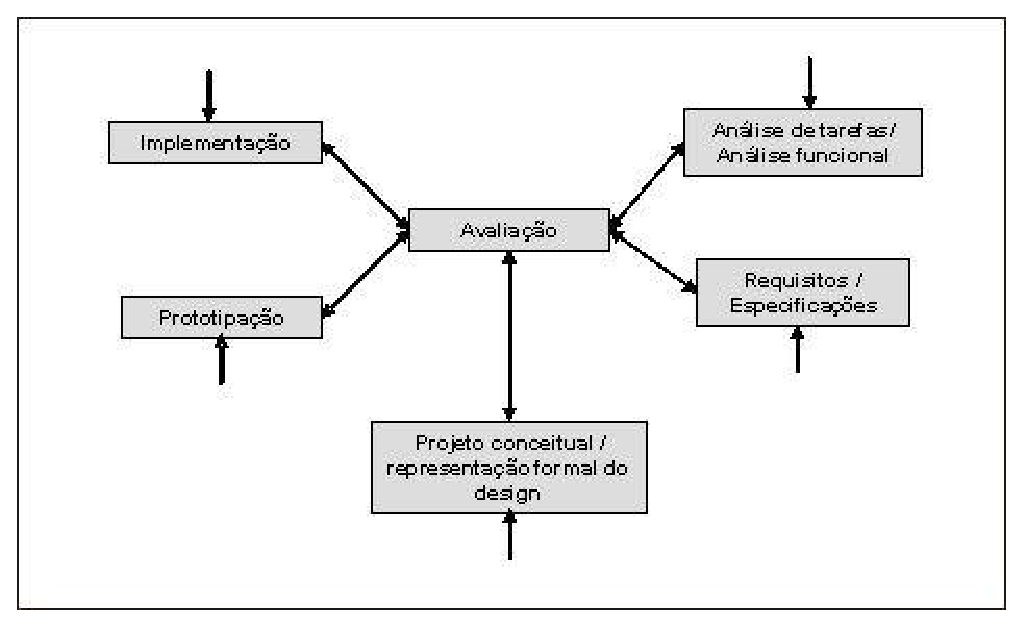
\includegraphics[keepaspectratio,scale=1.0]{figuras/ciclo_de_vida_estrela.eps}
		\caption{Ciclo de Vida Estrela}
	\end{center}
\end{figure}

Desta forma, as atividades são interconectadas, e é possível pular de qualquer uma para qualquer outra, contanto que se passe pela Avaliação antes. 